\documentclass[aspectratio=1610]{beamer}

\usetheme{unnslides}
\usefonttheme{professionalfonts}

\usepackage{listings}
\usepackage{graphicx}
\usepackage{caption}
\usepackage{cmbright}
\usepackage{fontspec}
\usepackage{unicode-math}
\usepackage{amsfonts}
\usepackage{subfig}
\usepackage{tikz}

\captionsetup[subfigure]{labelformat=empty}
\captionsetup[figure]{labelformat=empty}

\setromanfont{CMU Serif}
%\setsansfont{CMU Sans Serif}
\setmathfont{Latin Modern Math}
\setlength{\tabcolsep}{1pt}

\usepackage{polyglossia}
%\setbeamertemplate{itemize item}{\color{black}$\blacktriangleright$}

\DeclareMathOperator*{\argmax}{arg\,max}
\DeclareMathOperator*{\argmin}{arg\,min}
\DeclareMathOperator{\sign}{sign}
\DeclareMathOperator{\re}{Re}

\graphicspath{ {../images/}{img/} }

%set pages numeration
\newcommand\numbered{\setbeamertemplate{footline}{%
  \vspace{-10em}
   \raisebox{5pt}{\makebox[\paperwidth]{%
     \hfill\makebox[10pt]{%
       \usebeamerfont{footline}\usebeamercolor[fg]{footline}
       \insertframenumber}}}}}
\newcommand\unnumbered{\setbeamertemplate{footline}{}}

\title{Comparison of Several Stochastic and Deterministic Derivative-free Global Optimization Algorithms}
\author{\textbf{Vladislav~Sovrasov}}
\institute{Lobachevsky State University of Nizhni Novgorod}
\date{}

\begin{document}
\numbered
{
\unnumbered
\begin{frame}[noframenumbering,plain]
  \titlepage
\end{frame}
}

\begin{frame}
  \frametitle{Problem statement}
  \begin{columns}
    \begin{column}{0.5\textwidth}
      \begin{displaymath}
        \begin{array}{cr}\\
          \varphi(y^*)=\min\{\varphi(y):y\in D\}, \\
          D=\{y\in \mathbb{R}^N:a_i\leq y_i\leq{b_i}, 1\leq{i}\leq{N}\}
        \end{array}
      \end{displaymath}
      \(\varphi(y)\) is multiextremal objective function, which satisfies the Lipschitz condition:
      \begin{displaymath}
        |\varphi(y_1)-\varphi(y_2)|\leq L\Vert y_1-y_2\Vert,y_1,y_2\in D,
      \end{displaymath}
      where \(L>0\) is the Lipschitz constant, and \(||\cdot||\) denotes \(l_2\) norm in \(\mathbb{R}^N\)
      space.
    \end{column}
    \begin{column}{0.5\textwidth}
      \centerline{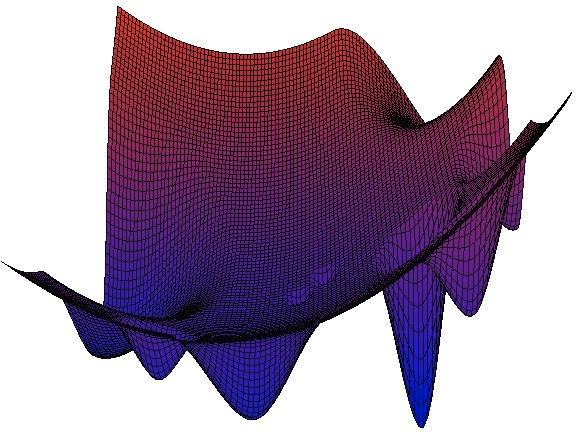
\includegraphics[width=0.9\textwidth]{img/gkls.png}}
    \end{column}
  \end{columns}
\end{frame}

\begin{frame}
  \frametitle{Methods}
  \begin{itemize}
    \item[$\square$] \textbf{Deteriminstic}:
    \begin{itemize}
      \item Have complicated internal structure in multidimensional case;
      \item Usually store and use the whole history of trials accumulated during search;
      \item Under some assumptions convergence to the global solution is guaranteed.
    \end{itemize}
    \item[$\square$] \textbf{Stochastic}:
    \begin{itemize}
      \item Have relative simple internal structure;
      \item Require constant amount of memory to store internal state of some random process or individuals of population;
      \item Convergence is guaranteed in probabilistic sense only.
    \end{itemize}
  \end{itemize}
\end{frame}

\begin{frame}
  \frametitle{Methods}
  In this work considered the following solvers available in open-source:
  \begin{itemize}
    \item[$\square$] \textbf{Deteriminstic}:
    \begin{itemize}
      \item DIRECT, DIRECT$l$ (Gablonsky J. M. et al, 2001);
      \item AGS (Strongin R.G., 1978).
    \end{itemize}
    \item[$\square$] \textbf{Stochastic}:
    \begin{itemize}
      \item Multi Level Single Linkage (Alexander H. G. et al, 1987);
      \item StoGO (Madsen, Kaj at al, 1998);
      \item Differential Evolution (Storn, Rainer et al, 1997);
      \item Controlled Random Search (Price, W. L., 1983);
      \item Dual Simulated Annealing (Y Xiang et al, 1997);
    \end{itemize}
  \end{itemize}
\end{frame}

\begin{frame}
  \frametitle{Univariate Algorithm of Global Search}
  Optimization method generates search sequence \(\{x_k:x_k\in[a,b]\}\) and consists of the following steps:
  \begin{enumerate}
    \setlength{\itemindent}{.1in}
    \item[Step 1.] Sort the search information (one-dimensional points) in increasing order.
    \item[Step 2.] For each interval \((x_{i-1}, x_i)\) compute quantity \(R(i)\), called characteristic.
    \item[Step 3.] Choose the interval \((x_{t-1}, x_{t})\) with the greatest characteristic and
    compute objective \(\varphi(y(x^{k+1}))\) in the point chosen using the decision rule \(d\):
    \begin{displaymath}
      x^{k+1}=d(t)\in (x_{t-1}, x_{t})
    \end{displaymath}
    \item[Step 4.] If \(x_{t}-x_{t-1}<\varepsilon\) stop the method.
  \end{enumerate}
  \textit{\footnotesize	{Detailed description: Strongin R.G., Sergeyev Ya.D.: Global optimization with non-convex constraints. Sequential and parallel algorithms (2000), Chapter 7}}
\end{frame}

\begin{frame}
  \begin{center}
  \frametitle{Dimension reduction}
  Peano-type curve \(y(x)\) allows to reduce the dimension of the original problem:
  \begin{gather}
    \lbrace y\in \mathbb{R}^N:-2^{-1}\leqslant y_i\leqslant 2^{-1},1\leqslant i\leqslant N\rbrace=\{y(x):0\leqslant x\leqslant 1\} \nonumber \\
    \min\{\varphi(y): y\in D\}=\min\{\varphi(y(x)): x\in [0,1]\} \nonumber
  \end{gather}
  \(y(x)\) is non-smooth function which continuously maps the segment \([0,1]\) to the hypercube \(D\).
  \begin{figure}[ht]
    \vspace*{-0.5cm}
    \subfloat{{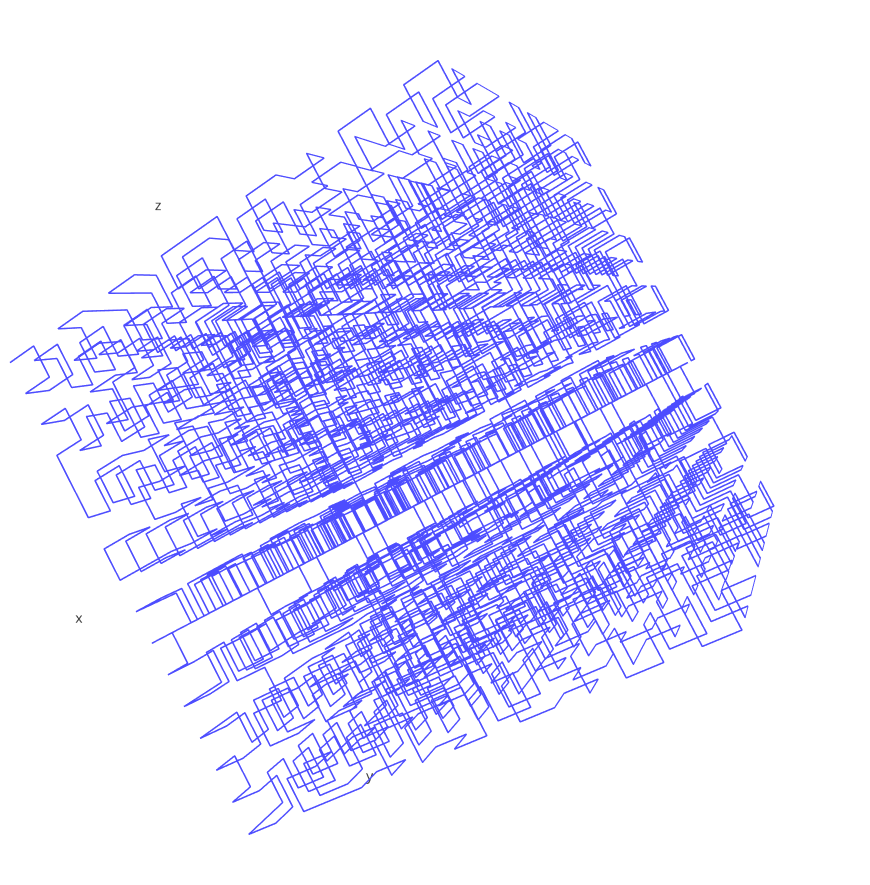
\includegraphics[width=.35\textwidth]{peano3d.png} }}
    \subfloat{{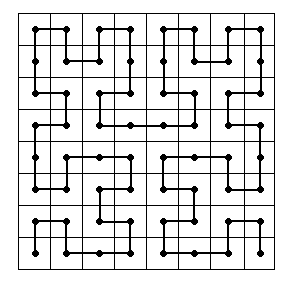
\includegraphics[width=.35\textwidth]{peano2d.png} }}
  \end{figure}
\end{center}
\end{frame}

\begin{frame}
  \frametitle{Hyperparameters tuning in AGS}
  AGS selects the best intervals according to the following characteristic:
  \begin{displaymath}
    R(i)=\Delta_i+\dfrac{(z_i-z_{i-1})^2}{(rH)^2\Delta_i}-2\dfrac{z_i+z_{i-1}}{rH},1<i<k+1
  \end{displaymath}
  where $L$ is the current estimation of the Holder constant, $r$ is reliability coefficient.
  AGS is very sensitive to choice of $r$:
  \begin{itemize}
    \item low value can lead to fast convergence to a local minima
    \item high value leads to very slow convergence
  \end{itemize}
\end{frame}

\begin{frame}
  \frametitle{Hyperparameters tuning in AGS}
  In order to resolve the problem of choosing $r$ to some extent,
  let us use the following scheme:
  \begin{itemize}
    \item execute $q$ iterations of AGS with $r=r_{max}$;
    \item execute $q$ iterations of AGS with $r=r_{min}$;
    \item repeat the above steps either until convergence or until the allowed number of iterations are
  exhausted.
\end{itemize}
  Now we have 3 parameters instead of one, but the method is not so sensitive to them.
  Let $q=50\cdot\log_2(N-1)\cdot N^2$, $r_{min}=3,\:r_{max}=2\cdot r_{min}$ in all the future experiments.
\end{frame}

\begin{frame}
  \frametitle{Test problems}
  \begin{columns}
    \begin{column}{0.5\textwidth}
      Generator GKLS (Gaviano, M. et al, 2003) was employed to construct 8 sets of 100 test problems:
      \begin{displaymath}
        \begin{matrix}
          f(x)=
          \left\{
          \begin{matrix}
          C_i(x), x \in S_i, i\in 2,\dots ,m \\
          \Vert x-T \Vert^2 + t, x\not\in S_2,\dots,S_m
          \end{matrix} \right.
        \end{matrix}
      \end{displaymath}

      The generator allows to adjust:
      \begin{itemize}
        \item the number of local minimums;
        \item the size of the global minima attraction region;
        \item the space dimension.
      \end{itemize}
    \end{column}
    \begin{column}{0.5\textwidth}
      \centerline{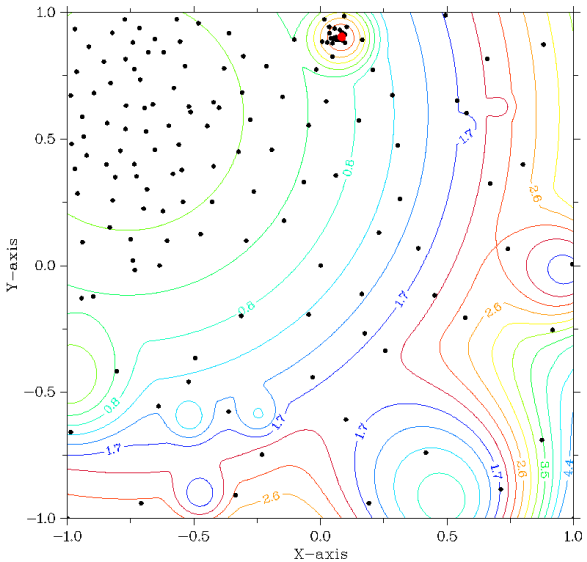
\includegraphics[width=0.9\textwidth]{gkls_color.png}}
    \end{column}
  \end{columns}
  Also one set of 100 pre-defined highly multiextremal functions (with 10-30 local minimums) was used.
\end{frame}

\begin{frame}
  \frametitle{Experimental setup}
  \begin{table}
  \begin{center}
  \caption{Trials limits and relative precision for the test problem classes}
    \begin{tabular}{|l|{c}|{c}|}
      \hline
    Problems class & Trials limit & $\alpha$\\
    \hline
    \(F_{GR}\) & 5000 & 0.01 \\
    \hline
    GKLS 2d Simple & 8000 & 0.01 \\
    \hline
    GKLS 2d Hard & 9000 & 0.01 \\
    \hline
    GKLS 3d Simple & 15000 & 0.01 \\
    \hline
    GKLS 3d Hard & 25000 & 0.01 \\
    \hline
    GKLS 4d Simple & 150000 & $\sqrt[4]{10^{-6}}$ \\
    \hline
    GKLS 4d Hard & 250000 & $\sqrt[4]{10^{-6}}$ \\
    \hline
    GKLS 5d Simple & 350000 & $\sqrt[5]{10^{-7}}$ \\
    \hline
    GKLS 5d Hard & 600000 & $\sqrt[5]{10^{-7}}$ \\
    \hline
    \end{tabular}
    \label{tab:limits}
  \end{center}
  \end{table}
\end{frame}

\begin{frame}
  \frametitle{Experimental setup}
  \begin{table}
  \begin{center}
  \caption{Class-specific parameters of the optimization algorithms}
    \begin{tabular}{|l|{c}|{c}|{c}|}
      \hline
      & AGS & CRS & DE\\
    \hline
    \(F_{GR}\) & \(r=3\) & popsize=150 & mutation=(1.1,1.9), popsize=60 \\
    \hline
    GKLS 2d Simple & \(r=4.6\) & popsize=200 & mutation=(1.1,1.9), popsize=60 \\
    \hline
    GKLS 2d Hard & \(r=6.5\) & popsize=400 & mutation=(1.1,1.9), popsize=60 \\
    \hline
    GKLS 3d Simple & \(r=3.7\) & popsize=1000 & mutation=(1.1,1.9), popsize=70 \\
    \hline
    GKLS 3d Hard & \(r=4.4\) & popsize=2000 & mutation=(1.1,1.9), popsize=80 \\
    \hline
    GKLS 4d Simple & \(r=4.7\) & popsize=8000 & mutation=(1.1,1.9), popsize=90 \\
    \hline
    GKLS 4d Hard & \(r=4.9\) & popsize=16000 & mutation=(1.1,1.9), popsize=100 \\
    \hline
    GKLS 5d Simple & \(r=4\) & popsize=25000 & mutation=(1.1,1.9), popsize=120 \\
    \hline
    GKLS 5d Hard & \(r=4\) & popsize=30000 & mutation=(1.1,1.9), popsize=140 \\
    \hline
  \end{tabular}
    \label{tab:params}
  \end{center}
  \end{table}
  \begin{itemize}
    \item in the DIRECT and DIRECT\(l\) methods, parameter \(\epsilon=10^{-4}\);
    \item in the SDA method, the parameter \(visit=2.72\).
  \end{itemize}
\end{frame}

\begin{frame}
  \frametitle{Results of different methods}

  \begin{table}
  \begin{center}
  \caption{Averaged number of trials executed by the methods for solving the test
  optimization problems}
  \resizebox{\textwidth}{!}{%
    \begin{tabular}{|l|{c}|{c}|{c}|{c}|{c}|{c}|{c}|{c}|{c}|{c}|}
      \hline
      & AGS & AGS-AR & CRS & DIRECT & DIRECT\(l\) & MLSL & SDA & DE & StoGO \\
    \hline
    \(F_{GR}\)     & 193.1 & 248.3 & 400.3 & \textbf{182.2} & 214.9 & 947.2 & 691.2 & 1257.3 & 1336.8 \\
    \hline
    GKLS 2d Simple & 254.9 & 221.6 & 510.6 & \textbf{189.0} & 255.2 & 556.8 & 356.3 & 952.2 & 1251.5 \\
    \hline
    GKLS 2d Hard   & \textbf{728.7} & 785.0 & 844.7 & 985.4 & 1126.7 & 1042.5 & 1637.9 & 1041.1 & 2532.2 \\
    \hline
    GKLS 3d Simple &  1372.1 & 1169.5 & 4145.8 & \textbf{973.6} & 1477.8 & 4609.2 & 2706.5 & 5956.9 & 3856.1 \\
    \hline
    GKLS 3d Hard   &  3636.1 & \textbf{1952.1} & 6787.0 & 2298.7 & 3553.3 & 5640.1 & 4708.4 & 6914.3 & 7843.2 \\
    \hline
    GKLS 4d Simple &  5729.8 & \textbf{4919.1} & 19883.6 & 7328.8 & 15010.0 & 41484.8 & 22066.0 & 6271.2 & 29359.2 \\
    \hline
    GKLS 4d Hard   &  13113.4 & \textbf{12860.1} & 27137.4 & 22884.4 & 55596.1 & 80220.1 & 68048.0 & 12487.6 & 58925.5  \\
    \hline
    GKLS 5d Simple &  \textbf{5821.5} & 6241.3 & 62921.7 & 5966.1 & 10795.5 & 52609.2 & 34208.8 & 20859.4 & 69206.8 \\
    \hline
    GKLS 5d Hard   &  \textbf{17008.6} & 21555.1 & 87563.9 & 61657.3 & 148637.8 & 138011.8 & 115634.6 & 26850.0 & 141886.5 \\
    \hline
  \end{tabular}}
    \label{tab:trials}
  \end{center}
  \end{table}
\end{frame}

\begin{frame}
  \frametitle{Results of different methods}
  \begin{table}
  \begin{center}
  \caption{Number of test optimization problems solved by the methods}
  \begin{tabular}{|l|{c}|{c}|{c}|{c}|{c}|{c}|{c}|{c}|{c}|{c}|}
    \hline
    & AGS & AGS-AR & CRS & DIRECT & DIRECT\(l\) & MLSL & SDA & DE & StoGO \\
  \hline
  \(F_{GR}\)     &  100 & 100 & 76 & 100 & 100 & 97 & 96 & 96 & 67\\
  \hline
  GKLS 2d Simple &  100 & 100 & 85 & 100 & 100 & 100 & 100 & 98 & 90\\
  \hline
  GKLS 2d Hard   &  100 & 97 & 74 & 100 & 100 & 100 & 93 & 85 & 77 \\
  \hline
  GKLS 3d Simple &  100 & 100 & 75 & 100 & 100 & 100 & 89 & 86 & 44 \\
  \hline
  GKLS 3d Hard   &  100 & 100 & 72 & 100 & 99 & 100 & 88 & 77 & 43 \\
  \hline
  GKLS 4d Simple &  100 & 100 & 74 & 100 & 100 & 94 & 82 & 68 & 72 \\
  \hline
  GKLS 4d Hard   &  100 & 100 & 60 & 99 & 99 & 94 & 73 & 55 & 69  \\
  \hline
  GKLS 5d Simple &  100 & 100 & 86 & 100 & 100 & 98 & 100 & 88 & 82  \\
  \hline
  GKLS 5d Hard   &  100 & 100 & 77 & 100 & 93 & 79 & 86 & 77 & 78 \\
  \hline
  \end{tabular}
    \label{tab:solved}
  \end{center}
  \end{table}
\end{frame}

\begin{frame}
  \frametitle{Results of different methods}
  \begin{figure}[ht]
    \centering
    \subfloat[4d Simple]{{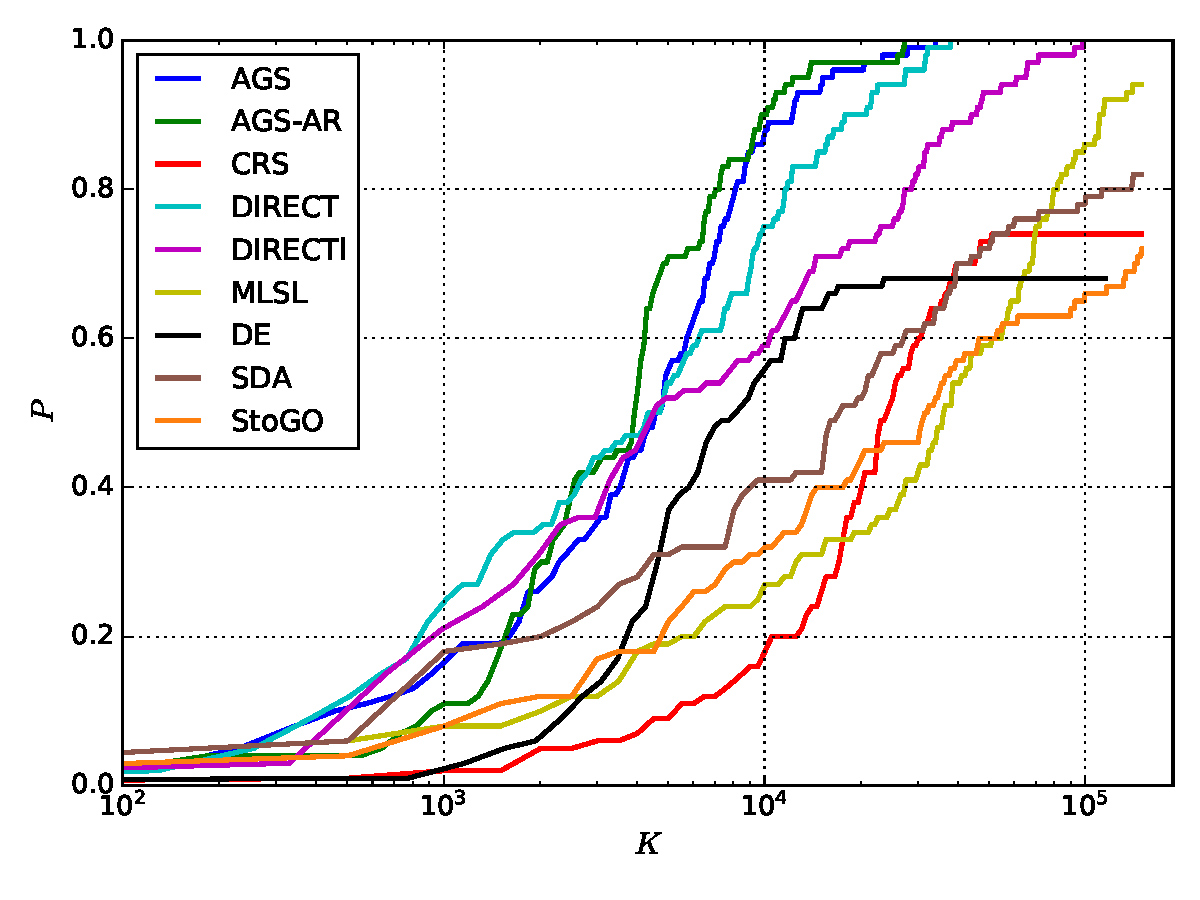
\includegraphics[width=.5\textwidth]{gklss4d.pdf}}\label{fig:s4d}}
    \subfloat[4d Hard]{{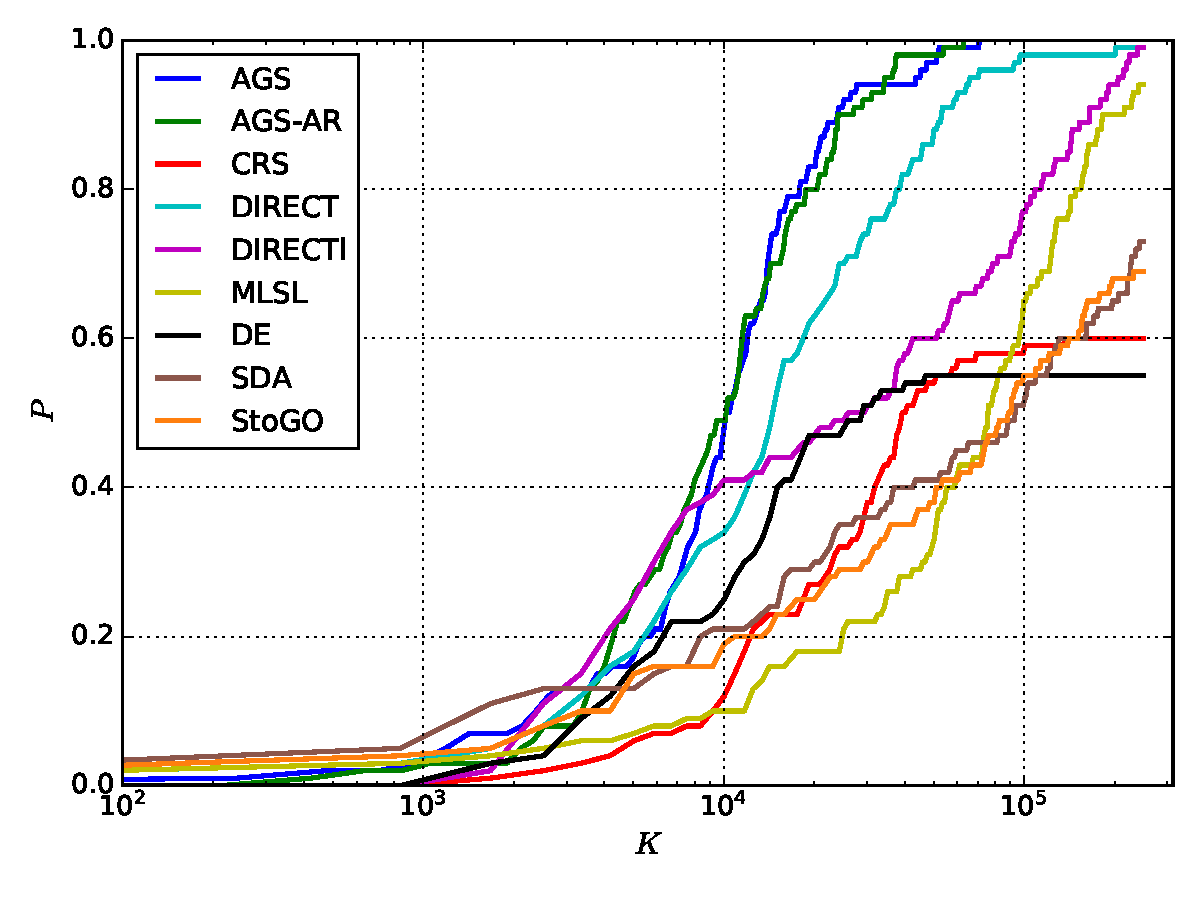
\includegraphics[width=.5\textwidth]{gklsh4d.pdf}}\label{fig:h4d}}
  \end{figure}
\end{frame}

\begin{frame}
  \frametitle{Results of different methods}
  \begin{figure}[ht]
    \centering
    \subfloat[5d Simple]{{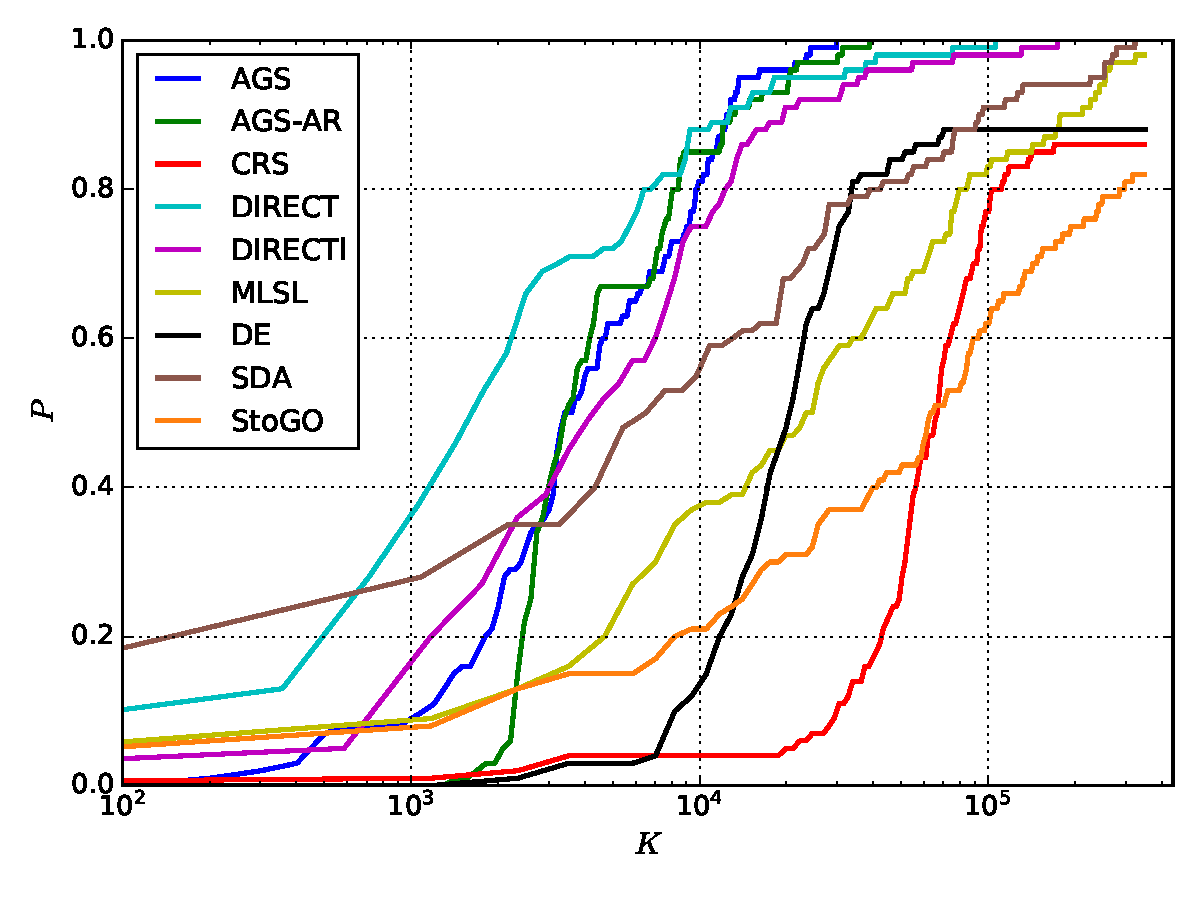
\includegraphics[width=.5\textwidth]{gklss5d.pdf}}\label{fig:s4d}}
    \subfloat[5d Hard]{{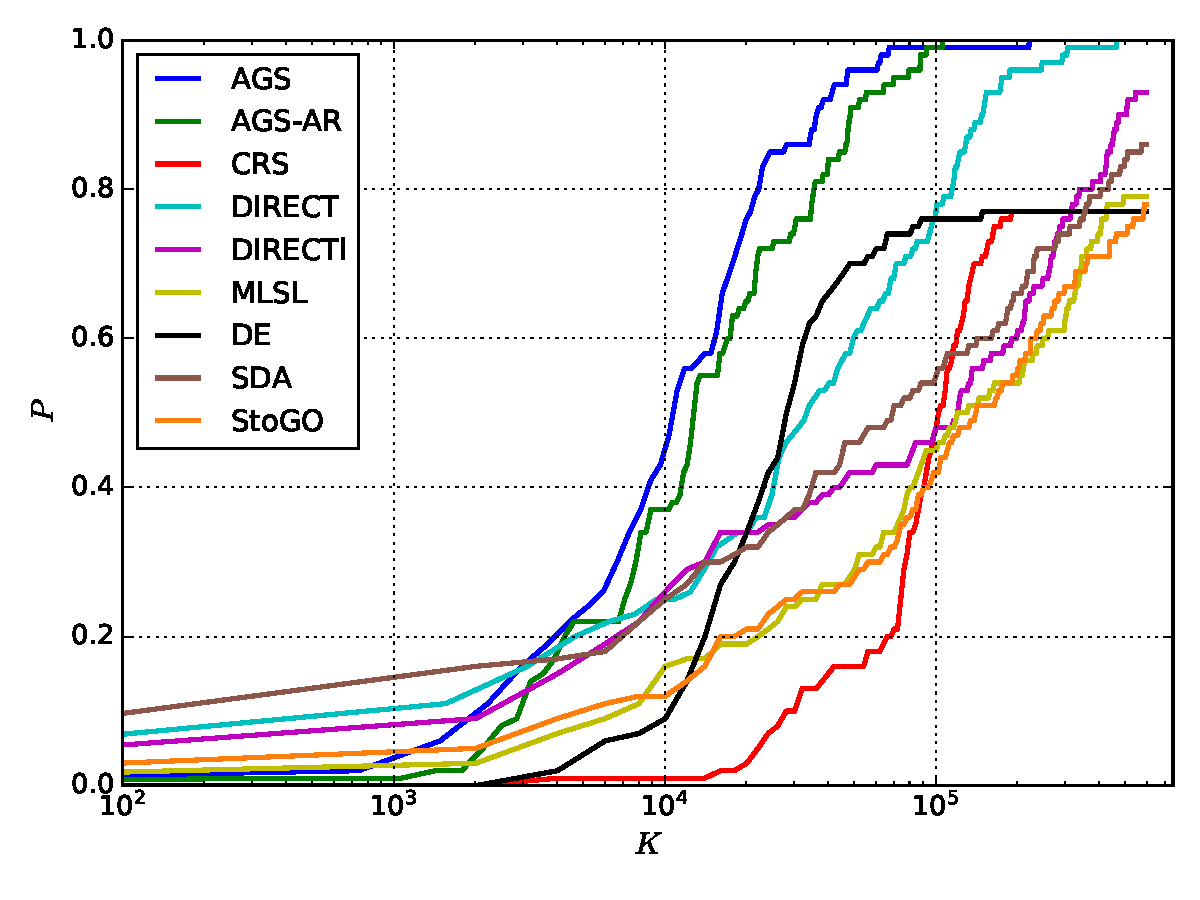
\includegraphics[width=.5\textwidth]{gklsh5d.pdf}}\label{fig:h4d}}
  \end{figure}
\end{frame}

\begin{frame}
  \frametitle{Robustness of the AGS-AR to hyperparemeters}
  \begin{figure}[ht]
    \centering
    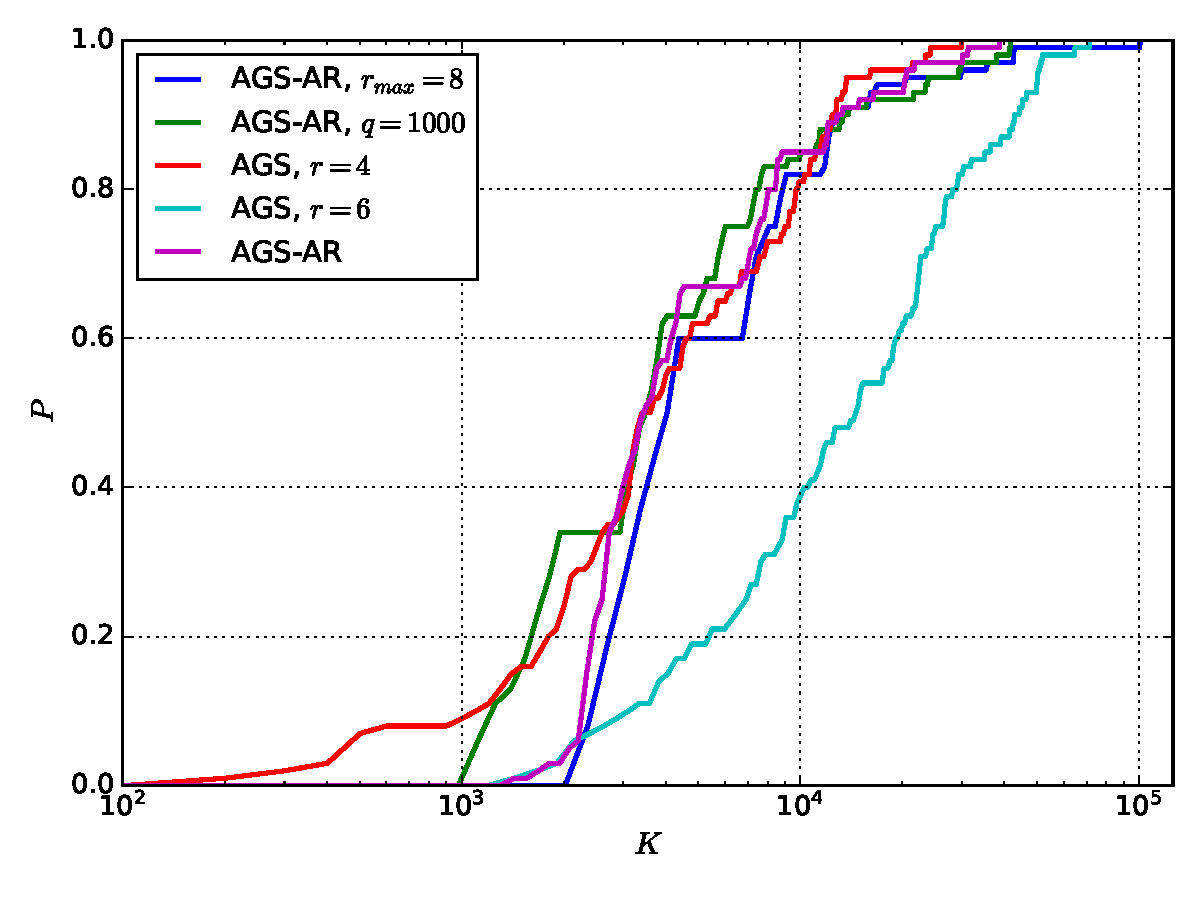
\includegraphics[width=.6\textwidth]{ar_stab.pdf}
    \caption{Operating characteristics of AGS and AGS-AR with different hyperparameters
    when solving problems from the GKLS 5d Simple class.}
    \label{fig:stability}
  \end{figure}
\end{frame}

\begin{frame}
  \frametitle{Conclusions}
    %Already done:
    \begin{itemize}
      \item The proposed modification of the stock AGS, AGS-AR allows to pay less attention to initial hyperparameter tuning and
      performs on-par with properly tuned AGS;
      \item AGS-AR method has demonstrated convergence
      speed and reliability at the level of DIRECT and exceeds many other algorithms, open-source
      implementations of which are available in web;
      \item considered stochastic optimization methods inferior to the deterministic ones in the convergence
    speed and in reliability. It is manifested especially strongly on more complex multiextremal
    problems.
    \end{itemize}
\end{frame}

{
\unnumbered
\begin{frame}{{}}
  \frametitle{Q\&A}
  \begin{center}
    \Large{Contacts:}
\vspace{0.5cm}

    sovrasov.vlad@gmail.com

    https://github.com/sovrasov
  \end{center}
\end{frame}
}
\end{document}
